\documentclass[UTF8,nofonts]{ctexart}
\date{\today}
\usepackage{geometry}
\usepackage{fancyhdr}
\usepackage{amsmath}
\usepackage{algorithm2e}
\usepackage{graphicx}
\setCJKmainfont{微软雅黑}
\setmainfont{微软雅黑}
\linespread{1.6}
\geometry{a4paper,left=3cm,right=3cm,bottom=3cm}
\pagestyle{fancy}
\fancyhf{}
\rfoot{\thepage}
\lhead{ }
\renewcommand\headrulewidth{0.8pt}
\begin{document}
\newpage
\vspace{1cm}
\section{Principles of Neural Science:Memory}
在加西亚.马尔克斯的著名作品百年孤独中,描述了这样的一种奇怪的瘟疫。这个瘟疫袭击了一个小村庄,染上瘟疫的人会逐渐的丧失记忆:首先是个人的过往记忆,然后是常见器物的名字和用途。一个人为了与这种瘟疫做斗争,在自己家的所有器物上都贴上便笺。但是随着词语和字母的认知能力的丧失,一切抗争都归为徒劳。
\par
这段离奇故事从某个角度上说明了学习和记忆在我们日常生活中的作用。学习指的是通过获得的知识来改变行为,而记忆指的是我们对这些知识的编码、存储以及检索的过程。在1861年Broca发现左额叶的后部(Broca区)损伤会导致语言功能的退化,这个发现引发了脑功能区的划分热潮。脑功能区的离散划分自然而然的引发了下面这个问题:这些功能区是不是通过记忆相连的呢?如果真的是通过记忆相连的话,记忆是通过一个记忆中心相连呢还是广泛的分布于各脑区?
\par
过去的几十年中,学习和记忆方面的研究有了很大的进展。当前章节中,我们将注重于下面三个方面的介绍:
\begin{enumerate}
\item 学习和记忆有很多类型,不同的类型有不同的认知性质,由不同的脑区控制。
\item 记忆可以分解为编码、存储强化、检索这三个过程。
\item 记忆的相关异常可以为学习和记忆的研究提供线索。
\end{enumerate}
记忆能够分解为两个维度:时间维度和存储结构。我们这里首先来探讨一下时间维度。
\subsection{长期记忆和短期记忆牵涉到不同的神经系统}
\subsubsection{短期记忆维持当前目标相关信息的呈现}
当提到记忆的时候,我们一般想起的是长期记忆,而忽视了短期记忆。但是,长期记忆是由短期记忆固化而来的。短期记忆,也叫做\textit{working memory},维持着容易消失的当前目标相关知识的呈现。人类的\textit{work memory}至少包含两个子系统:一个与语言(verbal)相关,一个与视觉(visuospatial)相关。这两个子系统由第三个子系统--\textit{executive control process} 调控。这个\textit{executive control process} 的主要功能是分配注意力,监控、操控及更新所存储的知识表达。
\par
语言子系统又包括两个子系统:一个用来存储语音相关的知识,一个用来回响接收的语音输入。神经生理学和神经成像的数据表明:语音知识的存储与后顶叶皮层有关,而回响则需要Broca区的参与。
\par
视觉子系统又与顶叶、内测颞叶、枕骨外皮层、前额叶、运动前皮层相关。至于这个视觉子系统是否可以分解为空间和物体这两个子系统,人们目前还没有定论。
\subsubsection{短期记忆会被选择性的转换为长期记忆}
在1950年代,学界从癫痫病人的切除治疗中获得了长期记忆是从短期记忆转换而来的惊人证据。这些病人的中颞叶的双侧海马和附近区域都被切除了,由此造成了这些病人的长期记忆形成障碍。这些病人中,最出名的就是代号为H.M.(为了维护病人隐私)的病人,心理学家Brenda Milner和外科医师William Scoville对这个病人做了长期的观察。2008-12-1,H.M.去世,他的真实姓名Henry Molaison才被披露出来。
\par
当时,病人H.M.为27岁的男性,7岁时由于自行车事故引起了脑部损伤,并因此忍受了10多年的不可治疗的颞叶癫痫。Scoville移除了这个病人的海马组织、杏仁核和双侧颞叶的multimodal association 区。在这个手术之后,H.M.的癫痫得到了很好的控制,但是他的记忆却损伤很大。但是,HM的记忆损伤非常特别,这种情况引起了人们的注意。
\par
HM仍然有正常的短期记忆(working memory),从几秒到几分钟不等。这个症状说明,中颞叶对于短期记忆来说并不是必须的。此外,HM对于手术之前的长期记忆仍然保持的很好。HM现在最主要的记忆困难是无法将新的短期记忆转换为长期记忆。他无法在记忆中维持刚刚认识的人、刚刚经历过的事情这些信息。当被要求背诵一个电话号码的时候,HM在几分钟之内仍然能够很好的完成这项任务。但是一旦将他的注意力转移,HM则会丧失对这个电话号码的记忆。HM并不是一个孤立的现象,所有经历过广泛双侧中间颞叶切除的病人都或多或少的会有短期记忆无法转换到长期记忆的症状。
\par
HM的重要性在于,他的功能损伤是证明记忆与中间颞叶(包括海马体)有关的第一个有效证据。考虑到海马体的大小比较大,人们不禁想知道:到底多大的损伤才会导致长期记忆困难?另外一个病人RB的临床病例表明,即使海马体只受损了一小部分,长期记忆仍然会受到很大的损伤。不同部位的损伤造成的后果可能不一样,例如海马体下面的前内鼻区(perirhinal)皮层损伤对于物体识别的影响比海马体上面的皮层损伤所造成的影响大。一些学者认为,海马体在空间认知方面的重要性比物体识别的重要性大得多。在人类身上的脑功能成像实验表明:右侧海马在涉及到空间信息记忆的行为中活动增强,而左侧海马在涉及到文字、物体及人物识别行为中活动增强。这个结论与临床上相关区域受损病人的症状相吻合。
\subsubsection{长期记忆可以分为显式记忆和隐式记忆}
在病人HM身上还观察到另外一个症状:并不是所有类型的长期记忆都完全受损,有些类型的长期记忆甚至是完全正常的。经历过类似手术病人大多也有这种症状。这种未受损的长期记忆大都来自于反射学习:即长期的重复某些活动从而得到了这个活动的长期记忆。比较生动形象的例子就是学自行车。但是反射学习并不仅仅限制在运动学习这一块,还包括habituation ,sensitization ,classical conditioning and operant conditioning。这类反射学习相关的记忆叫做隐式记忆(nondeclarative or procedural memory),这类记忆的检索完完全全是在意识无关的状态下进行的。而另外一种需要在意识作用下检索的记忆叫做显式记忆(declarative memory),它主要包括对于人、物和地点的事实知识。显式记忆是非常灵活的,多种不同环境的记忆片段可以一起链接起来。而隐式记忆则限制在特定场景下才能触发,也就是当时学习的环境条件。
\subsubsection{显式记忆拥有片段及语义形式}
加拿大心理学家Endel Tulving第一次提出了下面的观点:显示记忆可以被分类为两类-片段记忆(episodic memory)和语义(semantic)记忆。场景记忆是用来存储个人经历相关的知识,而语义记忆则是用来存储词汇和概念的意义。
\begin{figure}[h]
\centering
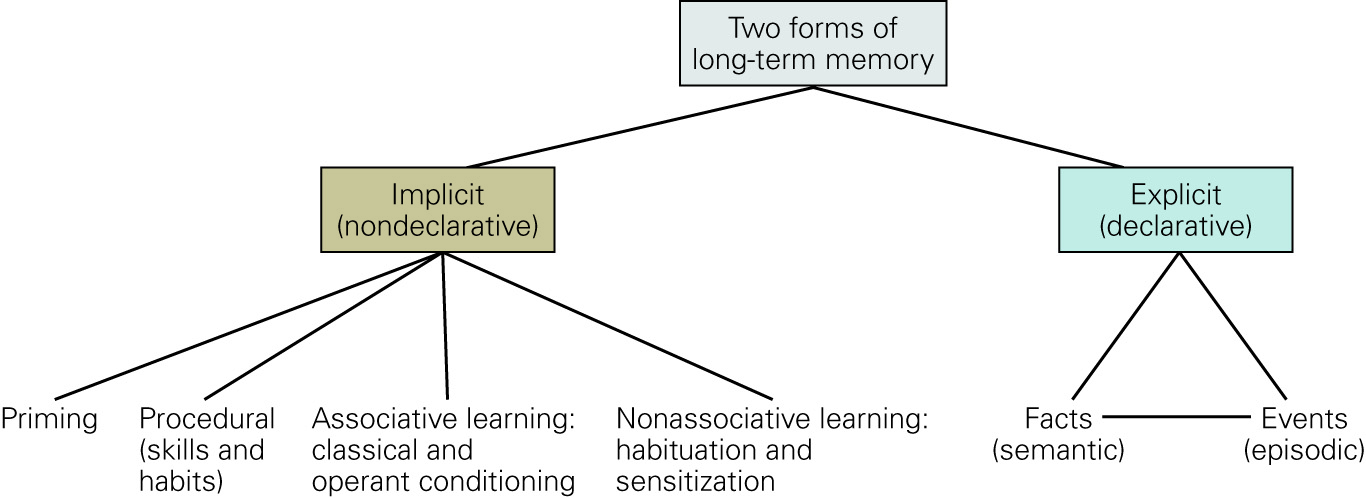
\includegraphics{Pic/6505_PNS5.jpg}
\end{figure}
对于显式记忆,我们还有如下的认识。
\begin{enumerate}
\item 大脑并没有一个单一的长期的显式记忆存储,而是分布在大脑的各个部分。这些不同部分的记忆检索可以被不同的方式独立触发,例如视觉、语音以及其他的感官信息。
\item 显式记忆至少有四个不同的信息处理过程: 编码(encoding),存储(storage),强化(consolidation),检索(retrieval)。这里我就不详细说了。
\end{enumerate}
\subsubsection{场景记忆依赖于中颞叶与相关皮层的交互}
临床失忆症病例表明,中颞叶的受损会影响在记忆上的所有四种操作:编码,存储,强化,检索,很难按照区域对功能进行定位。在PET和fMRI的帮助下,我们才能具体的观察各个不同区域在不同操作下的影响。fMRI表明:在涉及到深度编码(例如判断一个单词是具体还是抽象)时中颞叶的活动比浅显编码(例如是否一个单词是大写的还是小写的)时活动更强。左前额叶皮层在深度编码时,活动也会增强。这些证据表明前额叶与中颞叶在编码场景记忆是有很大的作用。后续的实验表明:场景记忆依赖于前额叶的认知控制过程和中颞叶的关联绑定机制之间的交互。
\par
中颞叶的不同的皮质区之间的交互对于记忆强化这个过程非常重要。HM的事例表明,老的记忆并不存储在中颞叶这里。根据Larry Squire等人的相关研究,中颞叶在记忆强化过程中只是当作一个临时存储区,这个存储区所存储的记忆会随着时间而衰退,而这些衰退的记忆会转移到皮质区。当记忆检索的时候,会同时检索这两个区域。失忆病人的症状与这个推论相吻合。
\par
\subsubsection{语义知识存储在不同的关联皮层以及检索依赖于前额页}
语义知识是我们对于这个世界的认识:包括客观事实、概念,以及词汇的意义。语义知识与场景知识的不同之处在于:语义知识与学习该知识所在的上下文无关。语义知识分布式的存储在大脑皮层中,包括颞叶的外侧和腹侧。不同的存储区域存储不同的信息,受损伤时只会影响特定的语义知识。Rosaleen McCarthy和Elizabeth Warrington 观察到拥有以下症状的病人:对于有生命的物体的知识受损,但是对于无生命的物体的知识保存完好。例如,一个病人把毛巾描述为“可以用来擦干身体的物体”,而把黄蜂描述为“一种会飞的鸟”。其他病人有刚好相反的症状。这些例子表明大脑是以概念原语来存储知识的,即 概念图谱。使用PET和fMRI的神经成像实验表明在正常人的大脑中知识是按照不同类别管理的。当人们被要求描述在照片中的动物时,左内侧颞叶活动增强。当被要求描述照片中的工具时,左前运动区和左中颞叶活动增强,这两个区域分别管理
使用物体时人运动的形式以及物体自己的运动形式。
\subsubsection{隐式记忆支持知觉启动(Perceptual Priming)}
隐式记忆存储那些下意识得到的知识。Priming是一种并不依赖于中颞叶的隐式记忆,在失忆症病人和正常人群中都有这种记忆。当前人们提出两种priming:\textit{Conceptual priming}和\textit{Perceptual priming}。Conceptual priming 提供任务相关的语义知识的快速访问,因为这些知识已经使用过了。而perceptual priming 则与具体的感觉信息有关。根据Tulving 和Schater ,perceptual priming 依赖于管理词语、对象的形式和结构感觉信息的皮质区。
对于皮层单一感觉区域的损伤会印象到该感觉模块相关的perceptual priming 。例如,右枕区广泛病变的病人无法正确处理词语的视觉priming,但是拥有正常的显式记忆。这个病例与HM刚好相反,说明priming的机制与显式记忆的机制是不同的。
\par
视觉priming总是伴随着高级视觉中枢的活动减弱。Randy Buckner 及其同事通过fMRI发现带外皮层(extrastriate cortex)的第一次打看到物体时的活动水平比之后看到同样物体的活动水平更高。这个发现也佐证了另外一个发现:左前额皮层的活动在概念priming时是减弱的。
\par
另外的一种隐式记忆是与学习相关的记忆,包括运动学习、感知学习以及习惯学习。运动学习这类记忆是通过重复的运动来得到的。这类运动感觉技巧的学习牵涉到基底节、小脑以及大脑皮层。帕金森与亨廷顿病人的基底节受损,从而无法学习运动技巧。小脑损伤也会造成类似后果。最后,熟练的运动行为都需要在相关的脑区的结构变化来得到固化,例如音乐家的手指部分。
\par
感知学习可以提高利用感官信息的能力,例如读取镜子中的逆向文本。通过不断的练习读取逆向文本,相关活动牵涉到的功能区也会发生改变。该开始的时候,读取活动会引起腹侧视觉处理区一级顶部皮层的活动增强。但是随着训练的进行,顶部皮层活动开始减弱,而左内侧颞皮层的活动开始增强。这个区域主要与视觉的表现形式有关,说明不断地练习读取逆向文本会把将文本逆转这个步骤消除,而直接从逆转文本中反射得到正向文本。即,相关的感觉学习从认知参与到自主反射的转变,所谓的习惯成自然。
\subsubsection{隐式记忆既可以是关联的也可以是非关联的}
所谓的关联记忆,指的是不同刺激之间或者刺激与行为之间的联系。而所谓的非关联记忆,指的是单个刺激的属性。非关联学习主要牵涉到单一刺激的长期作用,其结果主要有两类:习惯化(habituation)和敏感化(sensitization)。这两个词的意思很直接,这里就不再做多解释。在这两种情境下,刺激出现的时间并不重要。而在关联记忆中,两个刺激之间的先后关系很大程度的影响了关联记忆的强度。经典的条件发射牵涉到学习两个不同刺激之间的关系,而操作条件发射(operant conditioning)则涉及到学习一个行为的后果。
\subsubsection{经典条件反射牵涉到两个刺激之间的关联}
经典条件发射的喜闻乐见的例子就是驯狗大师巴普洛夫了。这个故事也是老生常谈,这里略去不提。这个经典条件发射牵涉到两个刺激:条件刺激(conditioned stimulus)和非条件刺激(unconditioned stimulus)。重复的条件刺激伴随着非条件刺激会引起脑对条件刺激的期望,也就是频发模式挖掘(frequent pattern mining)。这个关联确立之后,并不是永久的,如果多次非条件刺激缺失则会造成关联的extinction。更多的研究发现,这两个刺激的先后顺序并不重要,重要的是这两个刺激的时间间隔。
\par
脑的多个区域与关联学习有关。吹眼睛实验表明:大脑蚁(vermis)的损伤会导致条件刺激的无效化,但并不影响非条件刺激。
\subsubsection{操作条件反射牵涉到具体行为及其后果的强化}
所谓的操作条件发射比较通俗的说法就是尝试(trail and error) ,也就是对于具体行为的评价和反馈。人们普遍认为,虽然这两种反射的分型很明显,但是其底层机制应该是差不多的。越是与生存行为相关的刺激,大脑对这个刺激的记忆越强烈。其中最明显的就是味觉厌恶(taste aversion)。即使味觉条件刺激与呕吐相差的时间超过一小时,这两者的关联仍然很紧密。但是如果是视觉或者听觉刺激伴随着呕吐,则这两者的记忆关联则不是很强。即生物体并没有所谓的auditory aversion 和visual aversion。
\subsubsection{记忆相关的疾病和缺陷给予我们更多对于正常记忆的认识}
Daniel Schacter 把记忆相关的缺陷分为七类:transience ,absent-mindness ,blocking ,misattribution,suggestibility ,bias,persistence。这些单词的意思很直接,这里就不做太多解释。
\newpage
\subsection{隐式记忆存储的机制}
全书我们都在强调:所有的行为都是大脑作用下的结果,不管是正常还是不正常的大脑(所谓的行为学派)。我们所做的行为依赖于经验,而经验就是所存储的记忆。这些记忆从何而来,又是如何存储的。在本章,我们将尝试对隐式记忆的细胞和分子机制做相关介绍。
\begin{figure}[h]
	\centering
	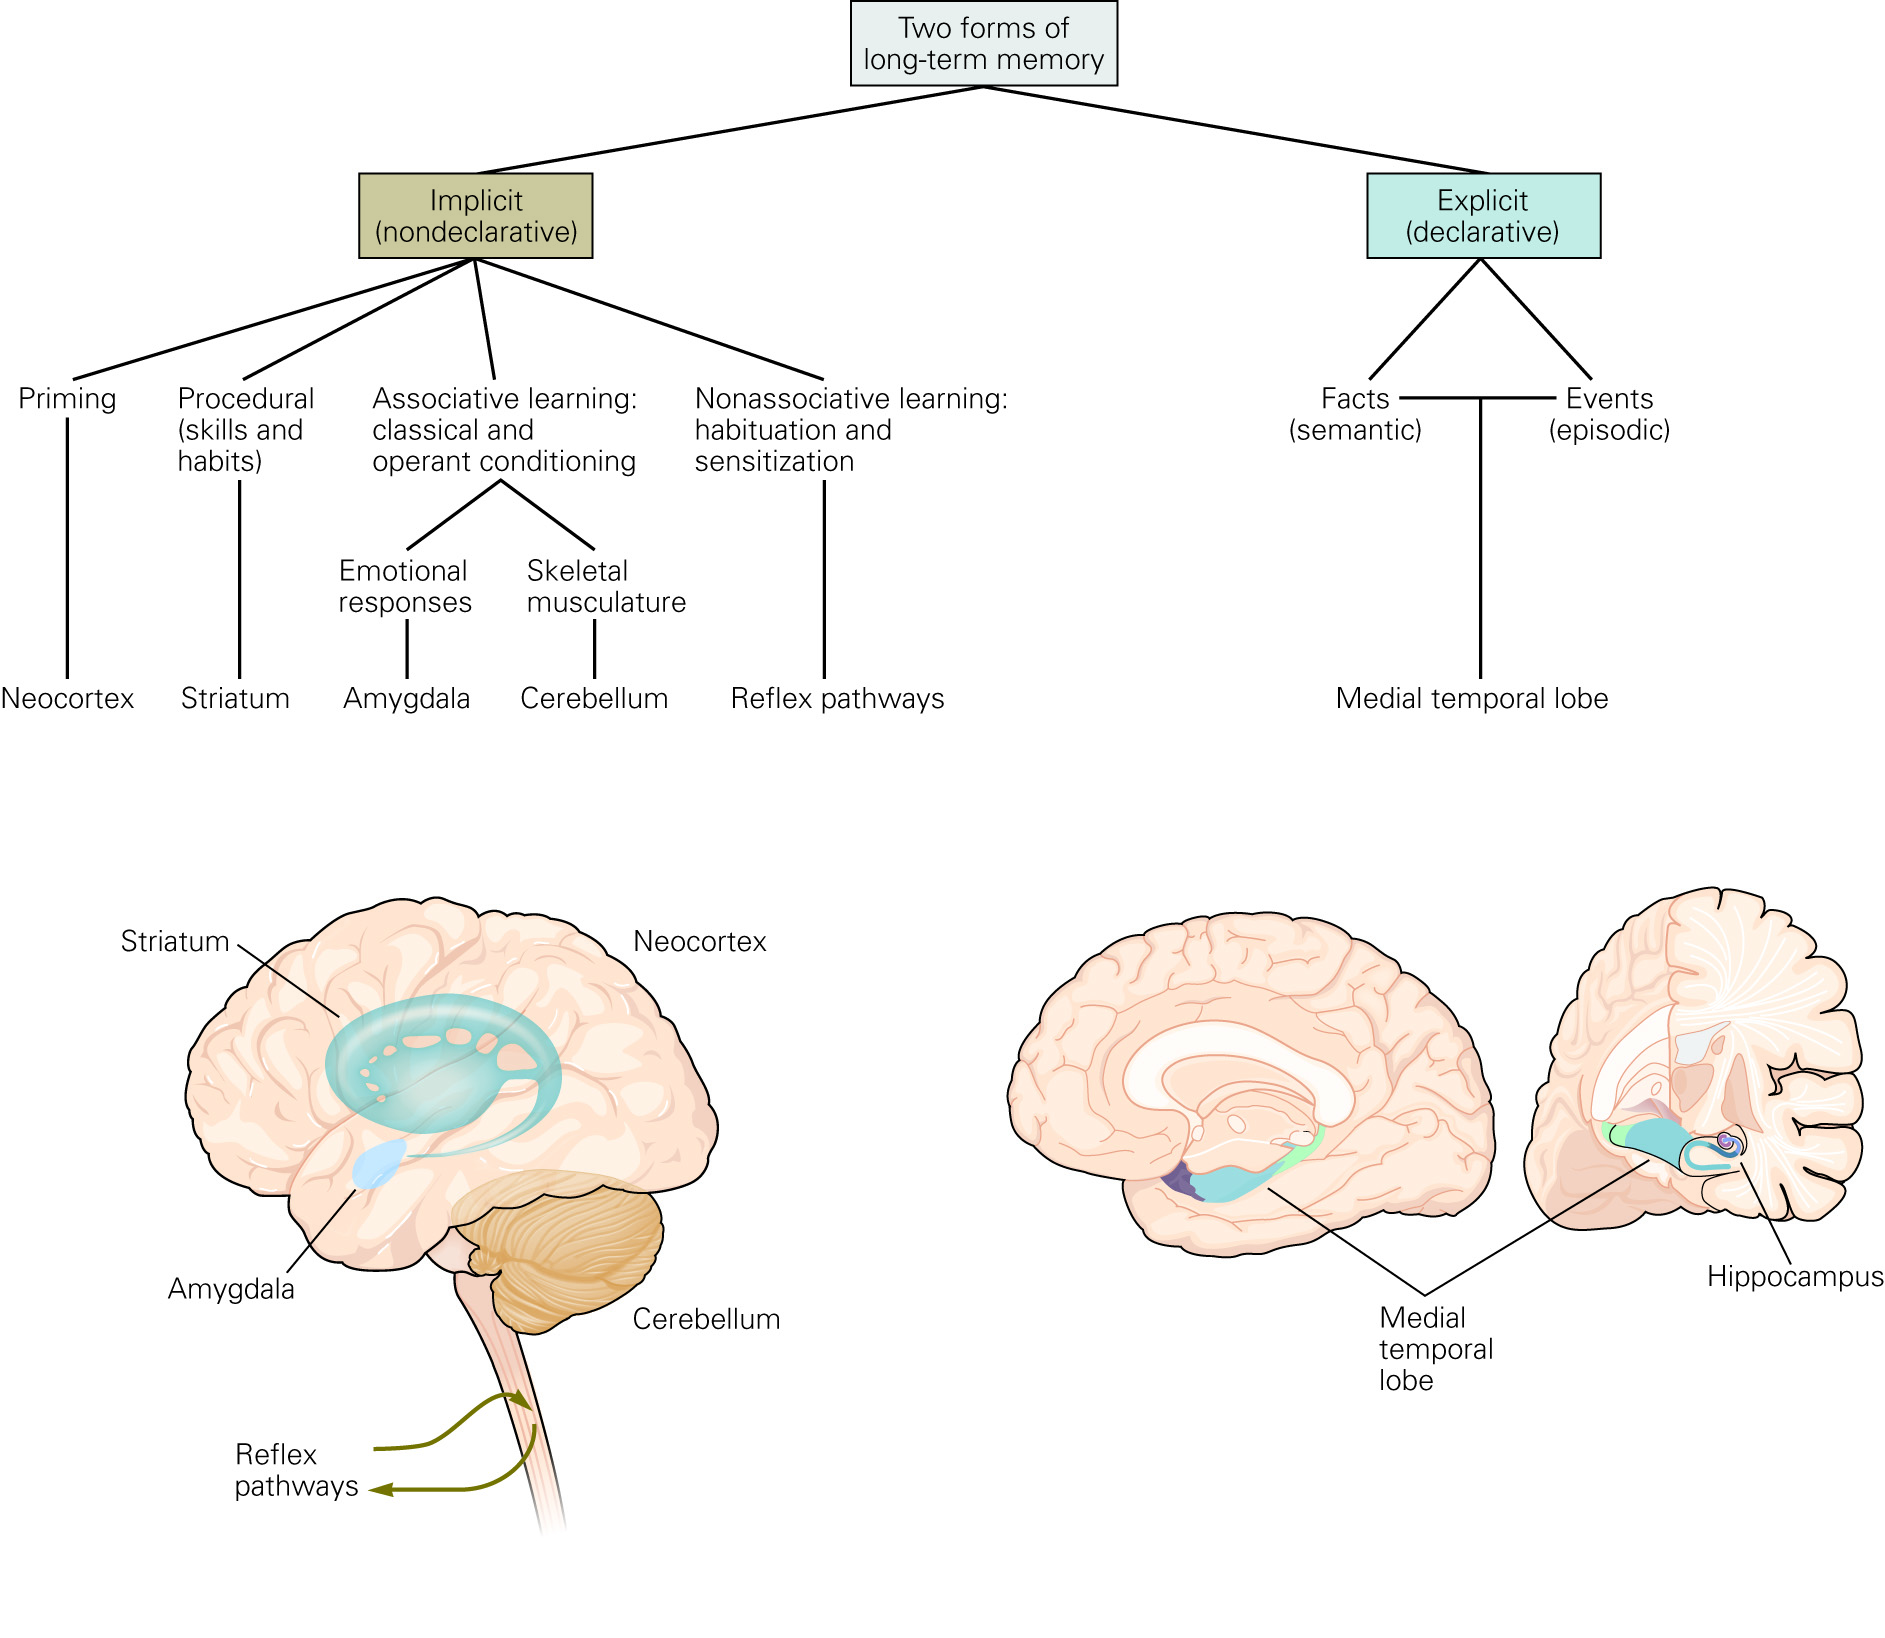
\includegraphics[scale=0.8]{Pic/6601_PNS5.jpg}
\end{figure}
\subsubsection{隐式记忆的存储与突触传输的效率相关}
在habituation,sensitization以及经典条件发射等隐式学习方面的研究提供了记忆存储基本机制的基础资料。这些学习在无脊椎动物和脊椎动物身上已经做了很详尽的研究,例如屈曲反射,恐惧应答以及眨眼。这些简单反射的学习会造成相应突触通路的效率改变。
\subsubsection{习惯化是突触传输中活动相关的突触前膜的抑制}
习惯化是最简单的一类隐式学习,它的生理学机制是被Charles Sherrington揭露的,当时他在研究猫的姿态和位置觉。Charles 观察到在重复的电刺激下,相应的反射应答的强度会减弱,他将这个现象称作 habituation。之后Alder Spencer和Richard Thomson 研究了这个现象的细胞机制。他们发现,在habituation期间,刺激部位局部的激动性中间神经元给予运动神经元的刺激会减弱。而感觉神经元与中间神经元之间的刺激强度保持不变。
\par
由于脊椎生物的中间神经元的构成非常复杂,很难分析其中的细胞机制。而海蜗牛(aplysia californica) ,由于其只有20000多个中央神经元的简单神经系统,被当作记忆研究的典型实验动物。海蜗牛有一个类似于屈曲反射的发射,而且这个反射的神经通路已经被细致的研究过了。通过触碰海蜗牛的肢体会触发机械门受体,从而引起感觉神经元的激动。感觉神经元的突触则释放出谷氨酸(glutamate),并引起中间神经元和运动细胞的快速的突触后动作电位(excitatory postsynaptic potentials),简称为EPSP。这些感觉细胞和中间神经元所产生的EPSPs在不同的时间和位置对运动细胞起作用,造成一个很强的刺激电流,并最终导致海蜗牛的快速应答。如果重复的进行刺激,由感觉神经元引起的中间神经元和运动细胞的单突触EPSP会逐渐减弱。此外,重复的刺激还会导致中间神经元与运动细胞突触间递质传输的减慢。这些因素,最终导致了反应应答的衰减。
\par
量化分析表明,在这个habituation的过程中,感觉神经元的突触前膜所分泌的谷氨酸数量会减少。谷氨酸的数量减少造成了突触小泡的数量减少,但是同时突触后膜对于谷氨酸的活性不变。由于这个过程并不涉及到其他细胞,所以这种衰减也被成为单突触抑制(homosynaptic depression)。这个抑制会持续好几分钟。
\begin{figure}[h]
	\centering
	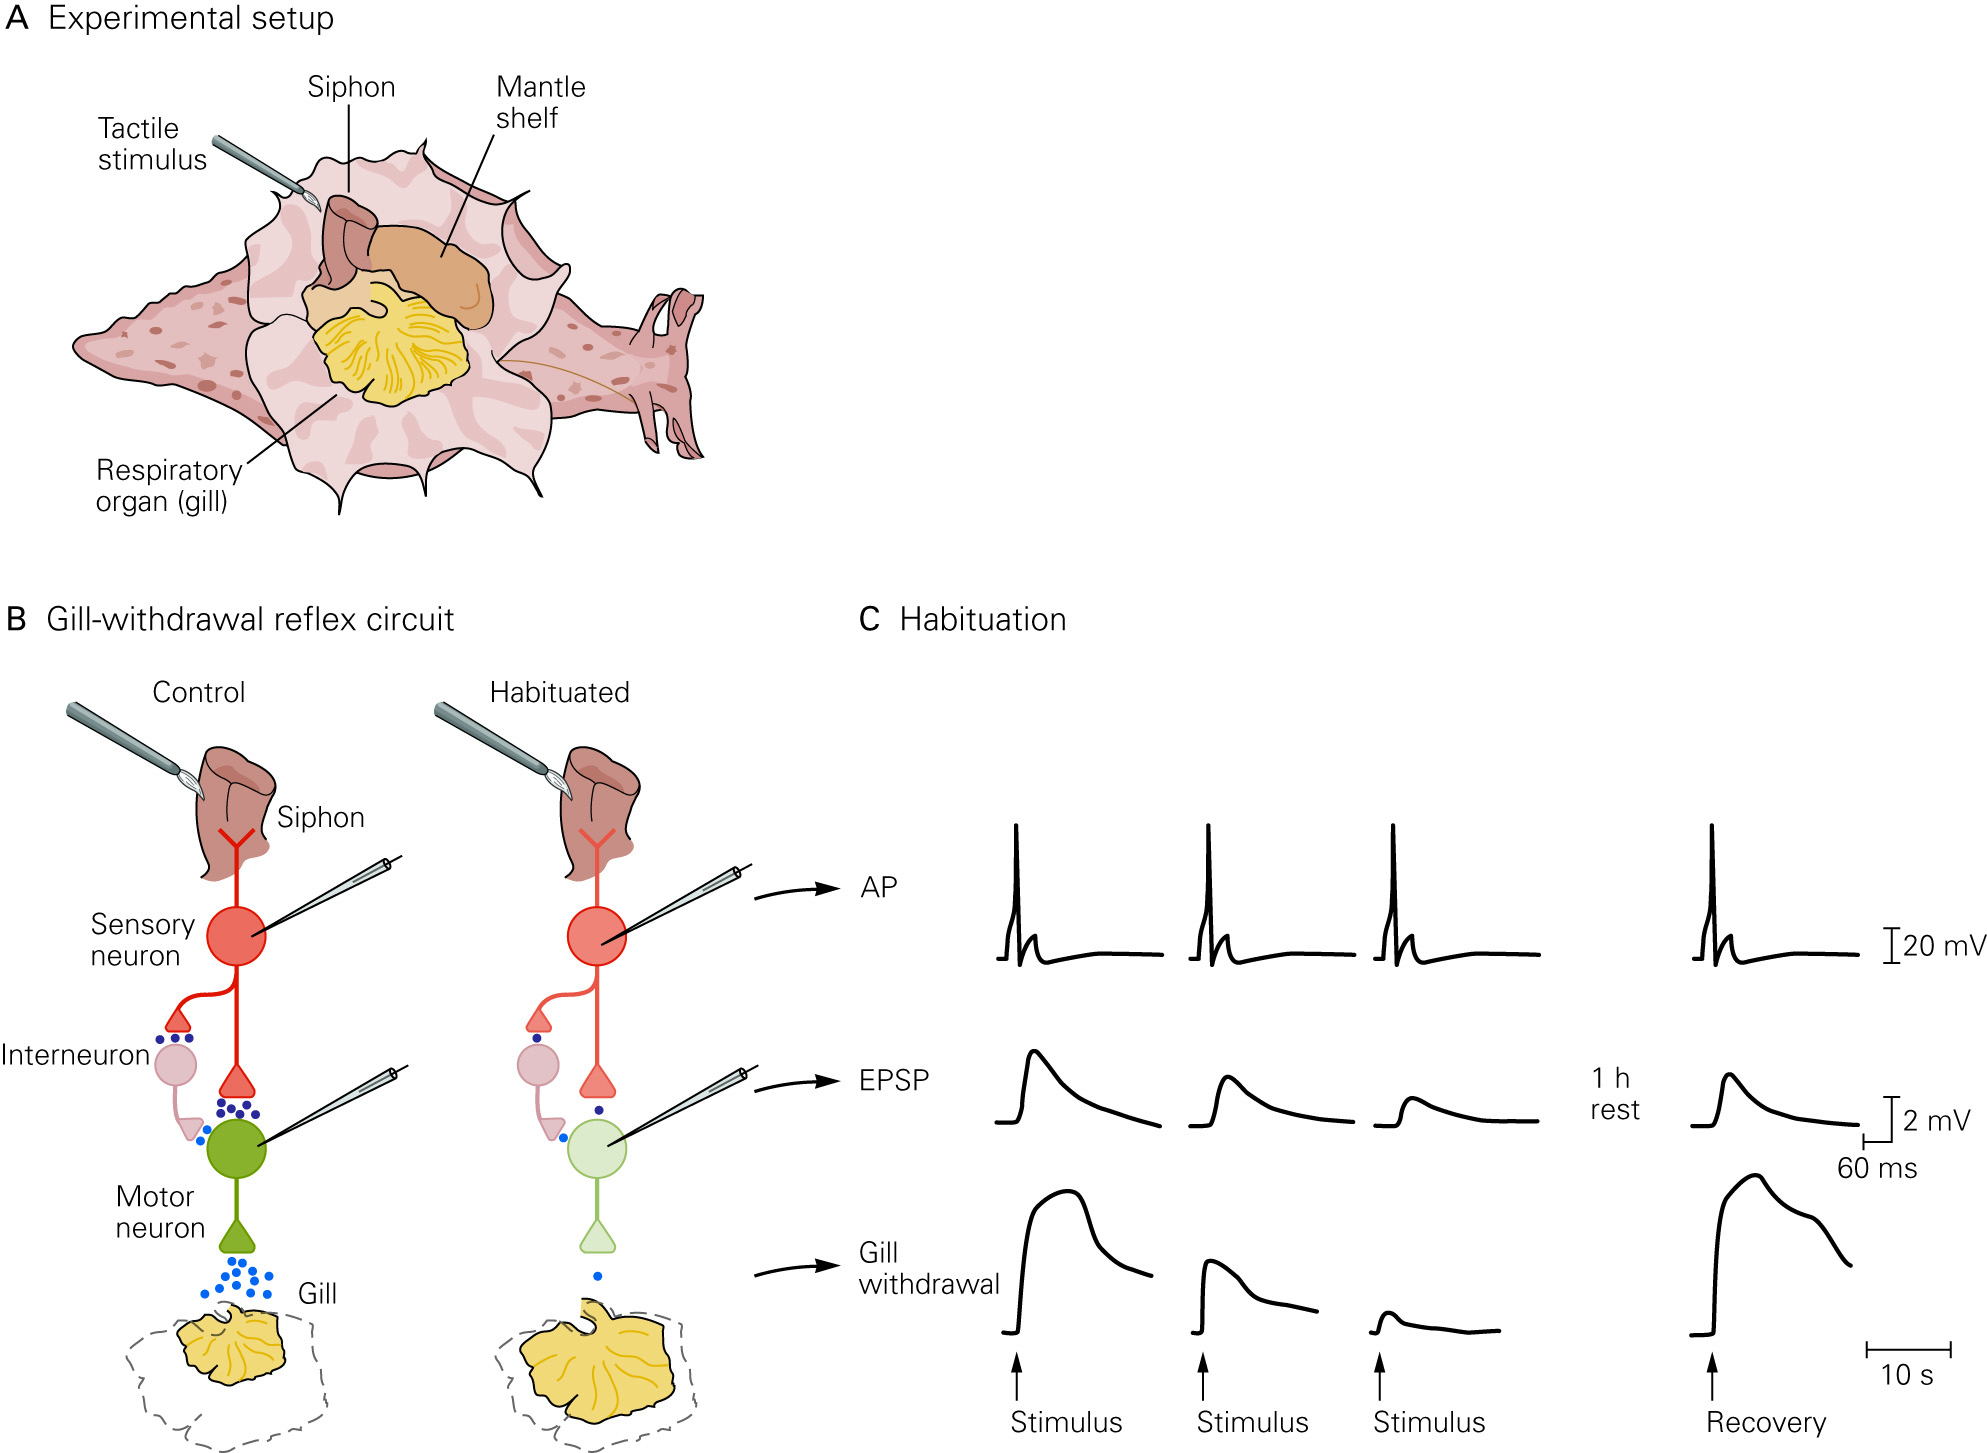
\includegraphics[scale=0.8]{Pic/6602_PNS5.jpg}
\end{figure}
\par
这种持续性的突触间功能强度的改变就是短期habituation的细胞机制。由于反射通路中会有多个点出现这种改变,所以相关的记忆也是分布的存储在整个反射通路中。多种生物实验证实了这种细胞机制也存在于其他生物中。
\par
这种突触间功能强度的改变会有多快,以及它会持续多久?在海蜗牛中连续的10个刺激会导致好几分钟的habituation。如果每10次刺激之间间隔几个小时或一天,连续刺激4次,则会造成持续时间长达3周的habituation。
\par
解剖学研究表明,长期的habituation是由于感觉和运动神经元之间的突触数量减少导致的。在没有habituation的动物中,90\%的感觉细胞会与运动细胞相连,而在经历过habituation的动物中则只有30\% 。突触数量的减少可以持续一周,有时三周之内都无法完全恢复。而敏感化则正好相反,突触数量会明显增加,这个将在后文中提到。
\par
并不是所有的突触修改的概率都是一样的。在海蜗牛中,一些突触的强度基本不随刺激的重复而变化,而另外的一些与学习相关的突触在少量的刺激下都可以长生持久而又强烈的突触强度增加。
\subsubsection{敏感化涉及到突触前膜的突触传输的增强}
当动物多次接触到有害刺激的时候,动物对这个有害刺激及其伴随刺激的反应强度都会增强,这个过程就叫做sensitization。和habituation一样,sensitization既可以是短期的,也可以是长期的。sensitization的细胞机制与habituation的细胞机制类似,只不过在数量上是正好相反的。
\par
至少三种模块化的中间神经元参与了sensitization,其中研究最透彻的神经元是以五羟色胺(serotonin)5-HT作为神经递质。5-HT能神经元在感觉神经元中分布非常的广,包括感觉细胞的突触前膜的轴轴突触。在物理刺激过后,中间神经元释放5-HT。这些5-HT会耦合到激动G蛋白受体,从而增加腺苷酰环化酶(adenylyl cyclase)的活性。腺苷酰环化酶活性增加的结果就是产生了第二信使cAMP(环磷酸腺苷),而cAMP则继续激活cAMP依赖的PKA(蛋白激酶A)。5-HT还激活第二种G蛋白偶联受体,并最终导致了磷脂的水解以及蛋白激酶c(PKC)的激活。
\par
由PKA及PKC调节的蛋白磷酸化从两个方面增强了感觉神经元的递质的释放。
\begin{enumerate}
	
	\item  PKA磷酸化钾离子通道,导致其关闭。这样增大了动作电位,并增强了钙离子通过电压门钙通道的内流。而钙离子会促进递质的释放。
	\item PKC引起的蛋白磷酸化直接增强递质的释放。
\end{enumerate}
这些由于5-HT释放所导致突触前膜的改变能够维持几分钟。重复的有害刺激下能够维持到好几天。
\begin{figure}
	\centering
	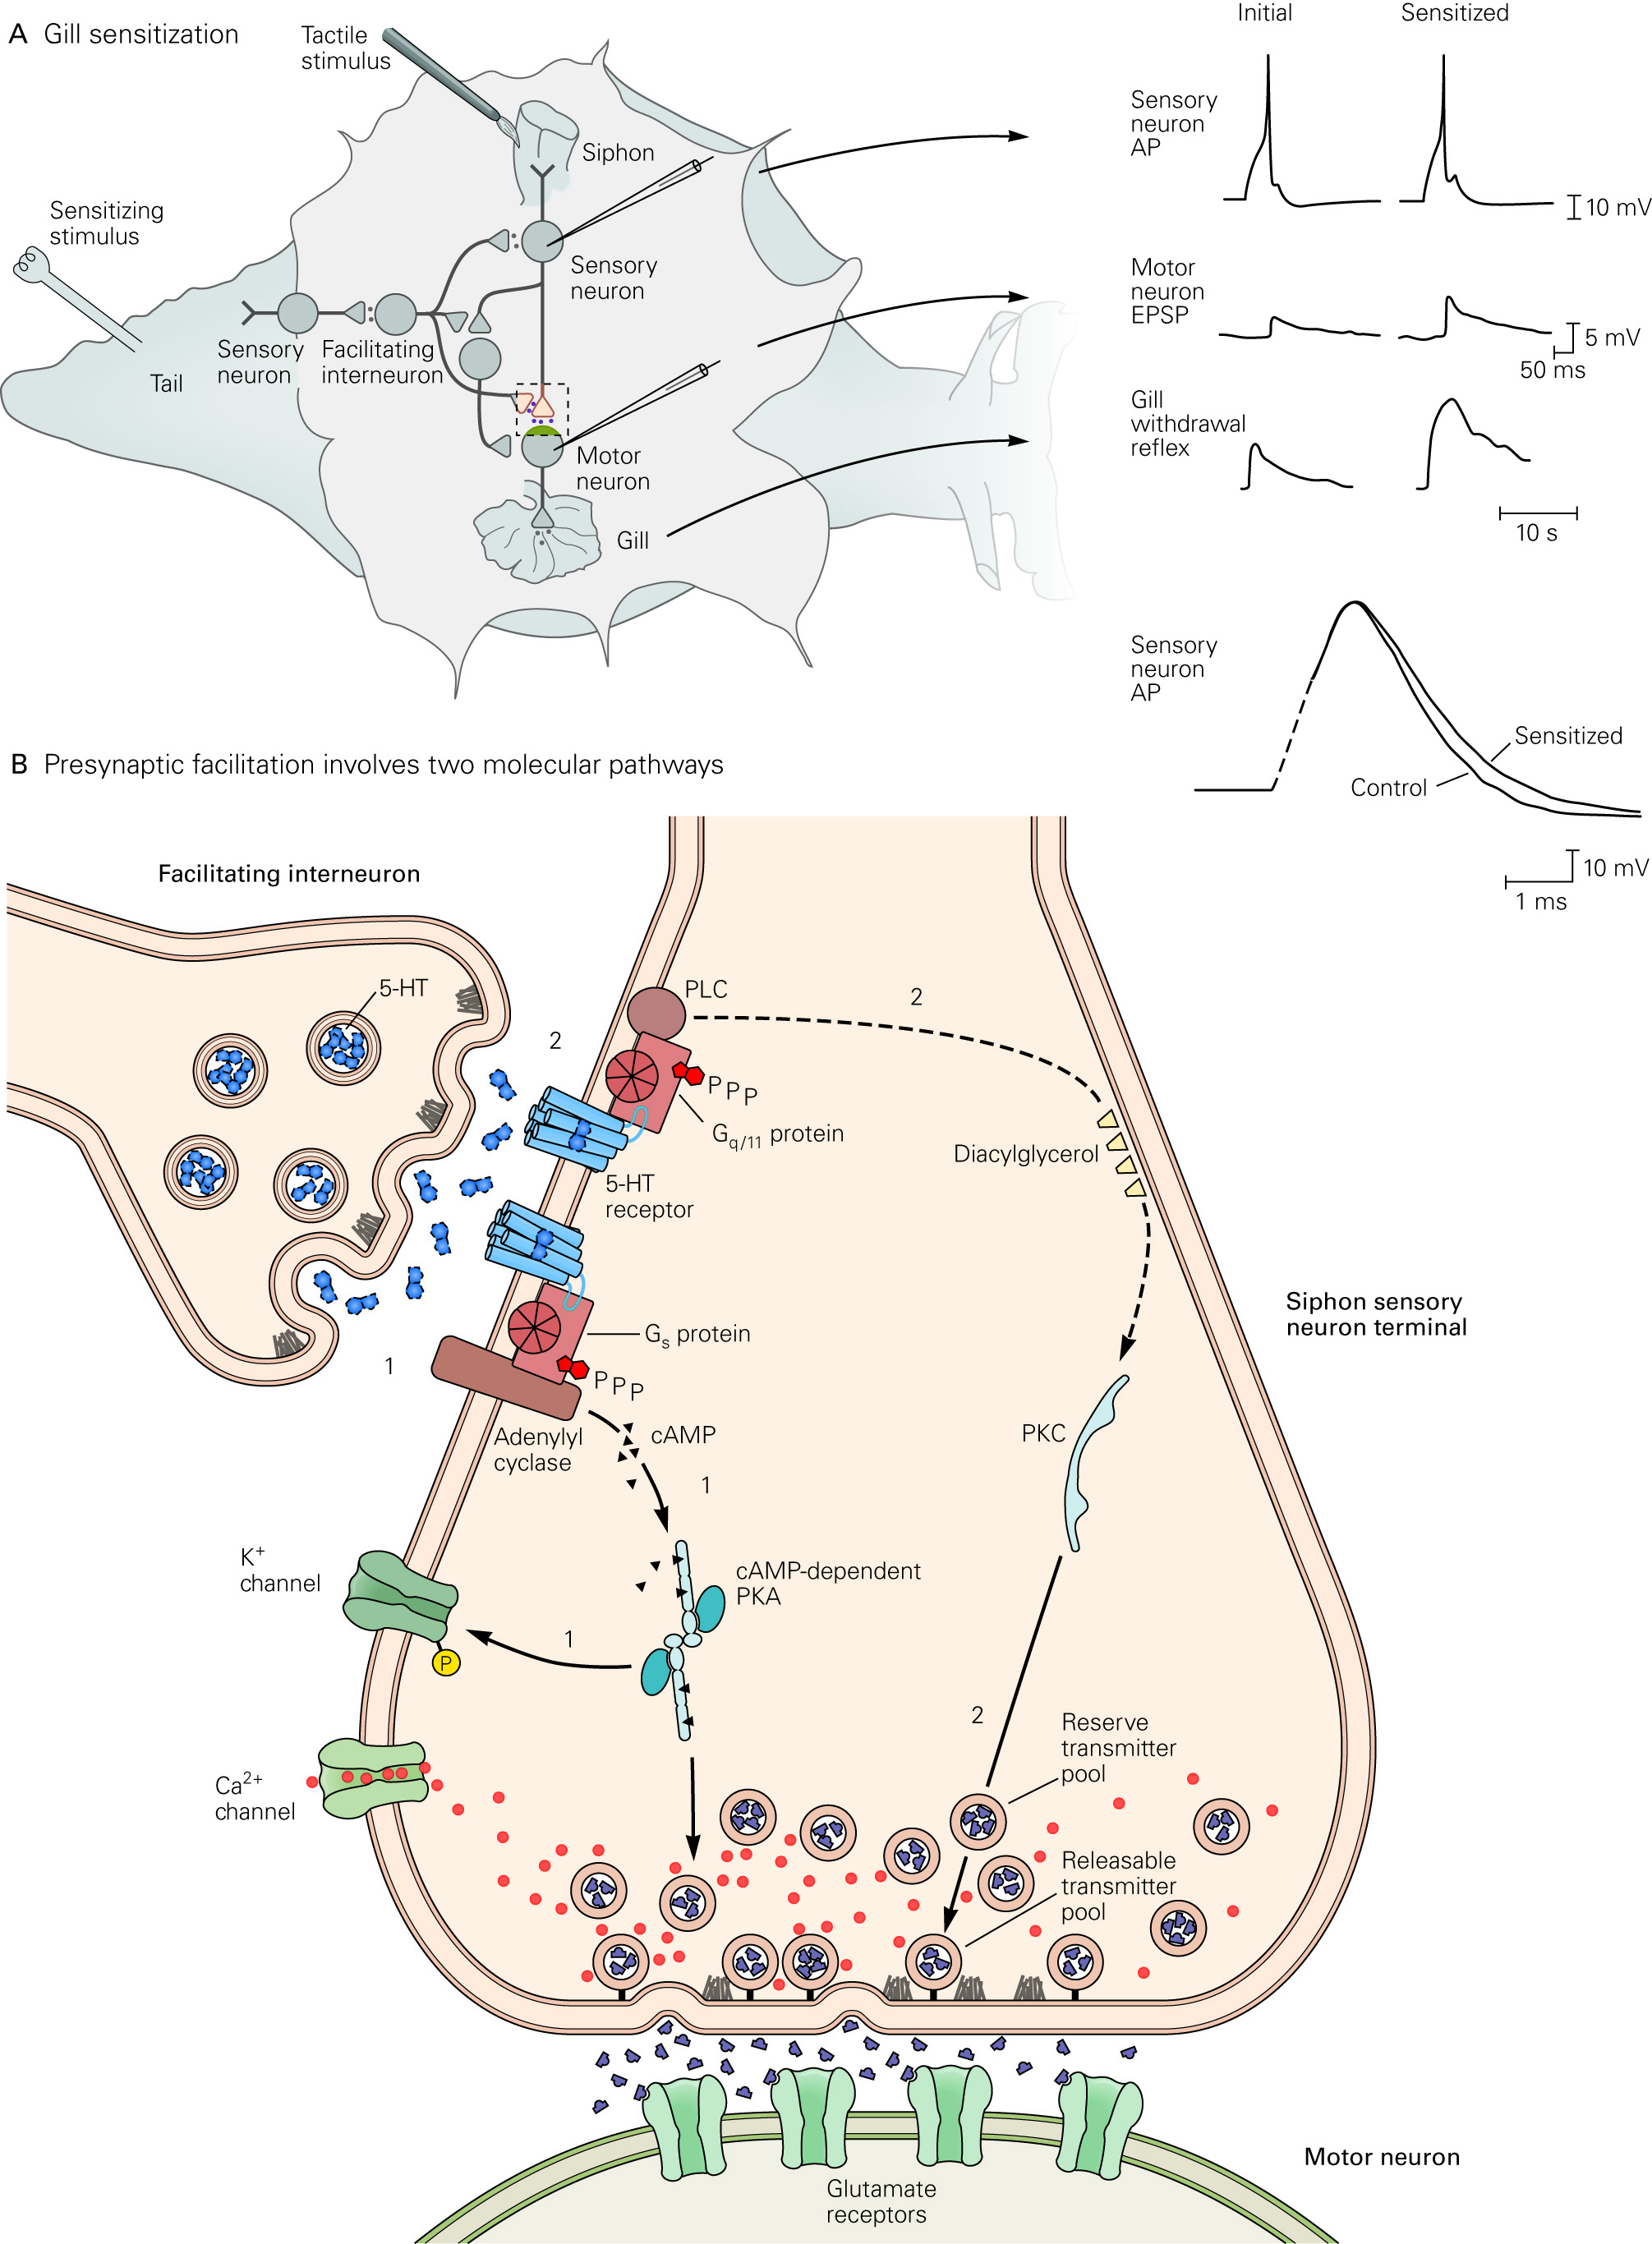
\includegraphics[scale=0.8]{Pic/6604_PNS5.jpg}
\end{figure}
\subsubsection{经典条件发射牵涉到突触前和突触后的突触递质释放的增强的协同作用}
经典的条件发射比学习更复杂,因为它牵涉到两个刺激。在海蜗牛的实验中,经过多次CS和US的协同刺激过后,单独CS刺激下所引发的活动甚至比单独US所引发的活动还强。而且实验中还发现,US和CS出现的时机也是非常重要的。为了达到有效刺激,CS必须出现在US之前的0.5s时间窗内。在此时间窗内,CS与US所引起的信号将会重合。强US刺激5-HT能中间神经元,并形成暂时的sensitization。但是,如果US是紧接着CS出现的话,中间神经元所释放的5-HT甚至能够激发更大的突触前易化作用,这个现象叫做活动相关的易化(activity-depedent facilitation)。
\begin{figure}[h]
	\centering
	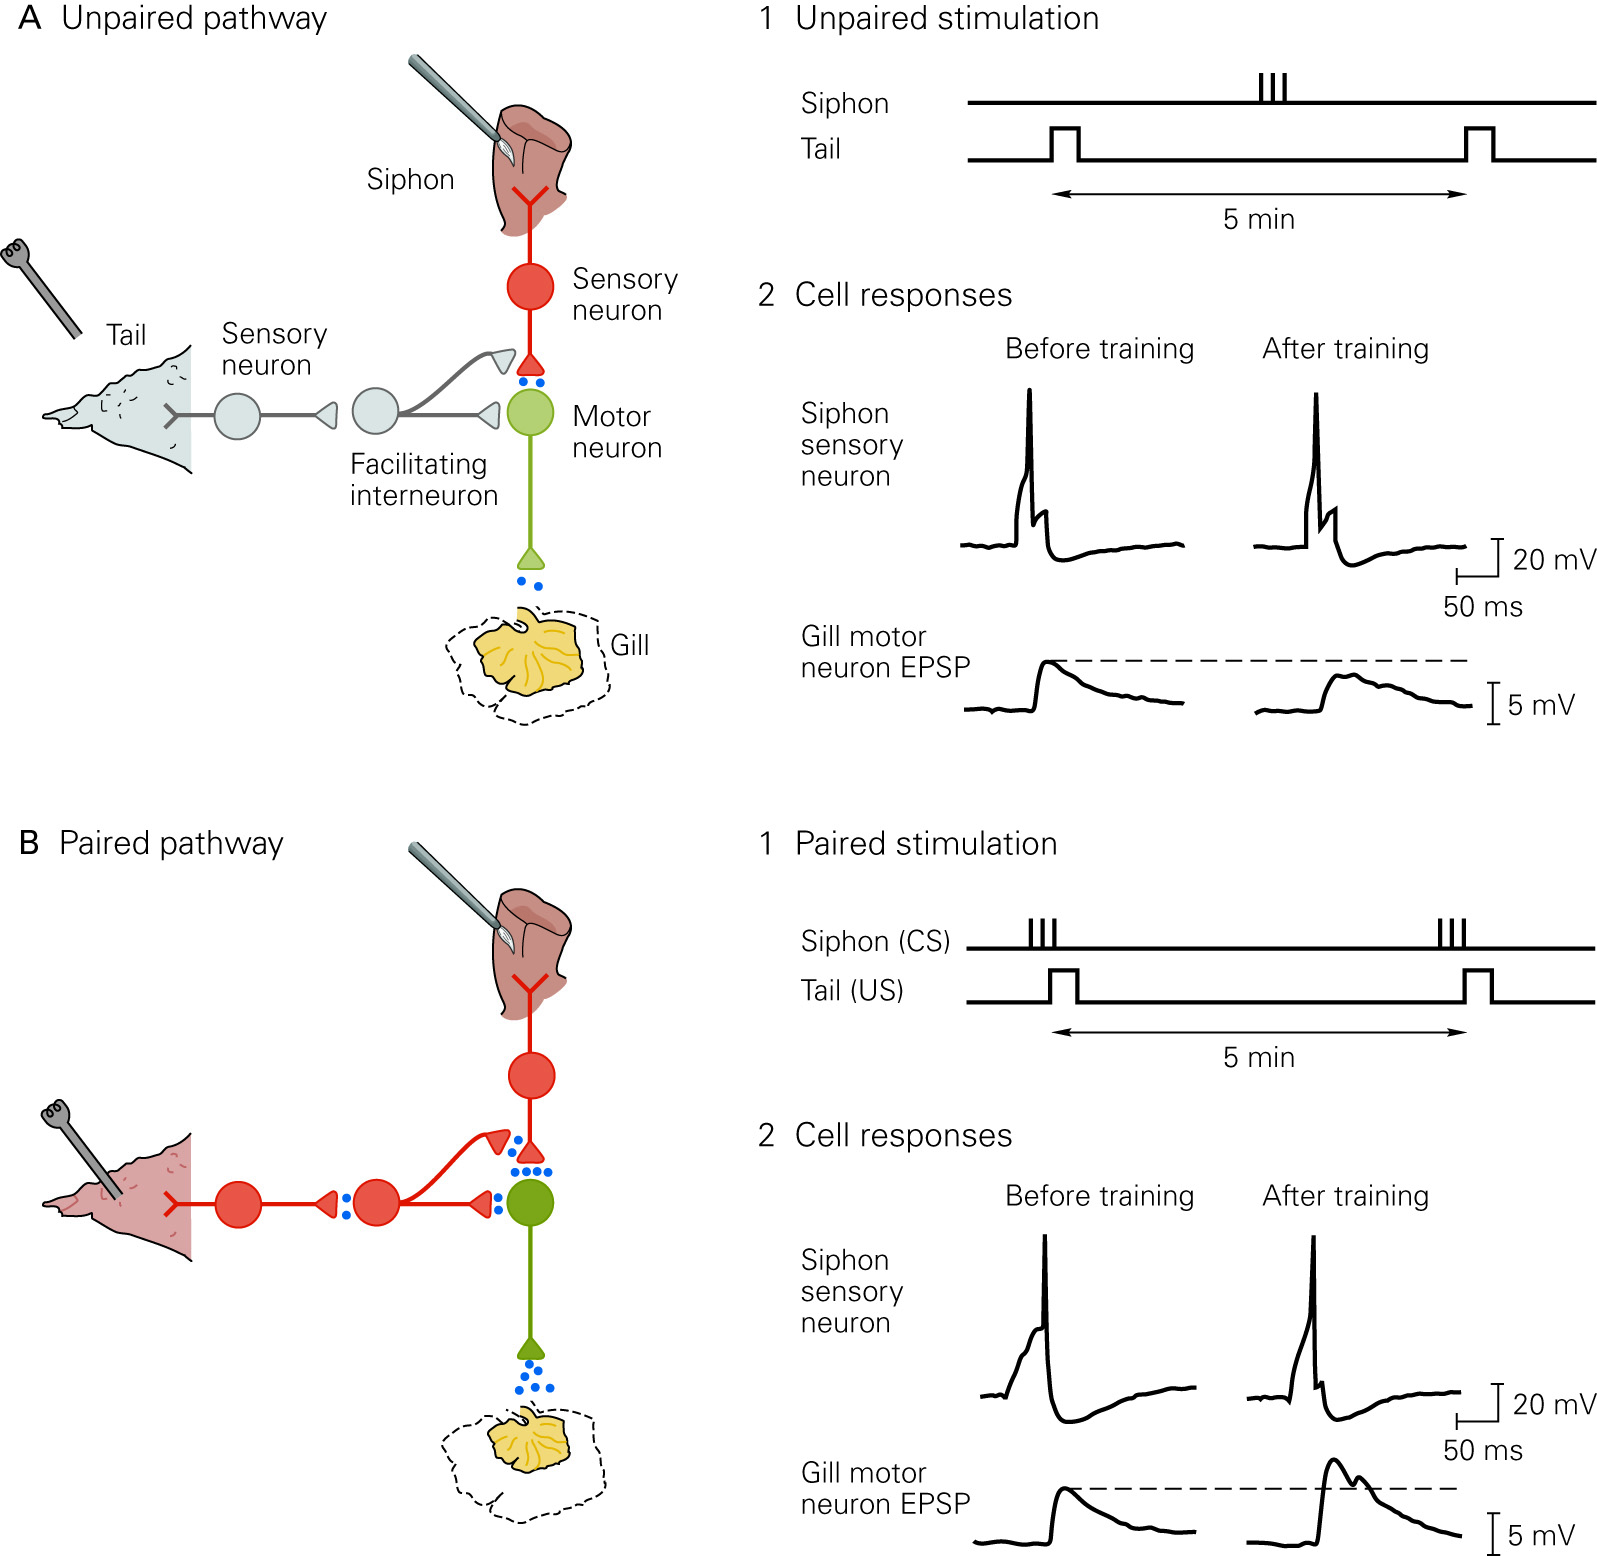
\includegraphics[scale=1]{Pic/6605_PNS5.jpg}
\end{figure}
为什么会出现这样的结果?在US刺激之后会释放5-HT,同时CS动作电位会引发感觉神经元突触前膜钙离子的内流。然后钙离子会绑定调钙素(calmodulin),然后这个复合物会绑定到腺苷环化酶。这样会促使腺苷环化酶对US刺激下生成的5-HT反应更加强烈。因此,cAMP的生成大大增强,并最终导致了突触前膜的易化。如果时间窗不重合或者时间顺序相反,则不会有这样的效果。
\par
因此,经典条件反射的sensitization在单突触通路上的细胞机制如前所述。其中腺苷环化酶起到了一个碰撞检测的作用,来检测US与CS之间是否重合。除了突触前膜的改变外,突触后膜也会做相应的改变,这里按下不表,留在67章讲LTP(long term potentiation)再去提。
\subsubsection{隐式记忆的长期存储会牵涉到染色结构和基因表达}
所有类型的学习最终都会牵涉到重复经验从短期记忆转变到长期记忆这一个过程。在海蜗牛中,这一个过程体现在长期的敏感化上。长期敏感化有着短期敏感化的所有特点,但是他还有自己的一个特殊的地方,就是长期敏感化会导致新的突触连接的生成。
\par
将短期记忆转换为长期记忆的过程,叫做固化(consolidation),这一个过程需要通路中的神经元合成mRNA和蛋白质。因此,特殊的基因表达对于长期记忆来说是必要的。这个记忆转换过程依赖于cAMP水平的长期升高,从而导致PKA的长期激活,并最终使得PKA的催化子单元进入到感觉神经的细胞核之中去。同时,它间接的激活了第二种蛋白激酶MAPK(mitogen-activated protein kinase)----丝裂原活化蛋白激酶,这个酶主要是用来调控细胞的有丝分裂。在细胞核内的PKA催化子单元会磷酸化,从而激活转录因子CREB-1(cAMP response element binding protein 1),这个转录因子会绑定到一个叫做CRE的启动子上。
\end{document}